\documentclass[10pt]{article} \usepackage[a4paper,left=0.8in,right=0.8in,top=0.4in,bottom=0.8in]{geometry} \usepackage{graphicx} 
\usepackage{url} 
\usepackage{datetime} 

\title{\textbf{CS296: Group 1 Project}\\{Gear Stop Clock driven by Perpetual Motion Machine}}
\author{ Siddharth Patel\\ 
120050001\\ 
\texttt{sidd@cse.iitb.ac.in} 
\and Ramprakash K\\ 
120050083\\ 
\texttt{ramprakash@cse.iitb.ac.in} 
\and Viplov Jain\\ 
120050084\\ 
\texttt{viplov@cse.iitb.ac.in}\\ 
} 
\date{\today} 

\begin{document} 
\maketitle 


\section{Introduction}In this document we will provide a detailed analysis of our CS296 project. It contains a system of gears kept in motion by a perpetual wheel that is run by a motor.
\section{Physics behind the simulation.}
\subsection{Perpetual Motion}
Perpetual motion is the action of the device that once set in motion would continue in motion forever, with no additional energy required to maintain it. Such devices are impractical in real life due to energy loses due to friction,however those machines which are close to perfect perpetual motion can be used to drive other engines such as clocks/turbines. This idea has been implemented to drive our mechanical clock. Even in Box2D, we were not able to simulate a perfect perpetual motion machine since the restitution of the bodies were to be less than 1 which meant that there would be energy loss. Hence, we had to attach a motor to keep it in motion.
\subsection{Perpetual Wheel}
The wheel we used in this project is the modified version of the Bhaskara Wheel which was one of the most earliest recorded man-made perpetual wheel. The idea was that the moment of inertia about the centre of the weights (spheres) that are descending is more than that of the weights that are ascending (since they are farther away from the centre) and hence, the wheel is supposed to experience continuous torque in a single direction.

\begin{figure}[ht!]
\centering
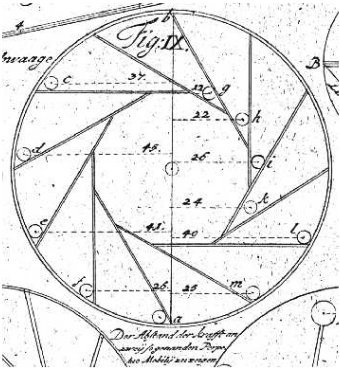
\includegraphics[width=0.5\textwidth]{images/pic.png}
\caption{Perpetual Wheel Design}
\end{figure}

\subsection{Gear Clock}
Mechanical clocks are made using gears, in which there are gears for each hand of the clock, and intermediate gears to connect them in appropriate ratios so that they rotate in the exact angular velocity as they denote.

\begin{figure}[ht!]
\centering
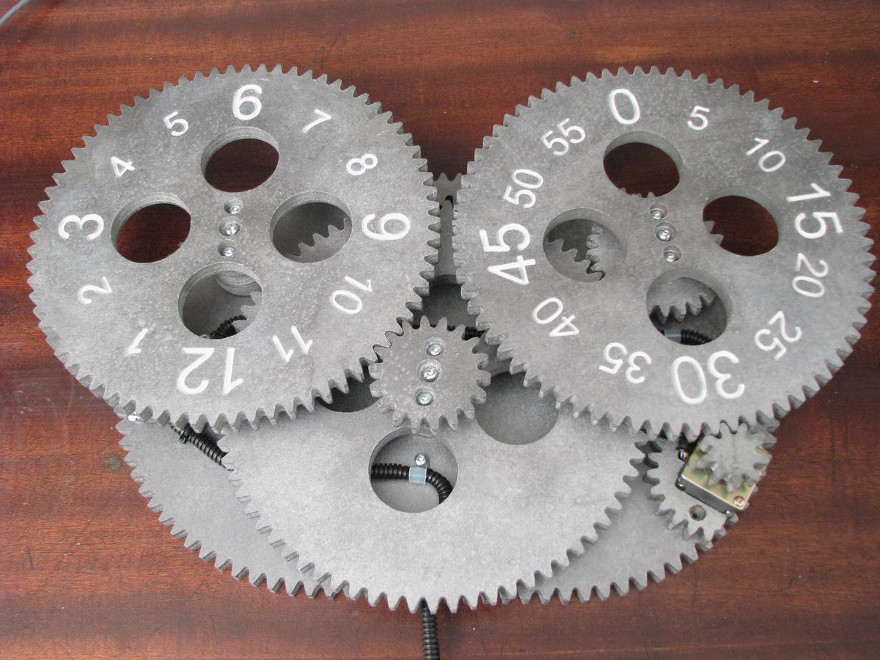
\includegraphics[width=0.5\textwidth]{images/gear_clock.jpg}
\caption{Gear Clock Design}
\end{figure}

Our perpetual wheel is attached to a motor that drives it at an angular speed of \textit{pi/5}.\\
We have a 10 tooth gear attached to our perpetual wheel that drives the 60 tooth gear denoting the seconds hand.\\
The 60 tooth gear has a 9 tooth gear attached to it which drives a 90 tooth intermediate gear.\\
The 90 tooth gear has a 12 tooth gear attached to it which drives the 72 tooth gear denoting the minute hand.\\
The 72 tooth gear has a 24 tooth gear attached to it which drives a 72 tooth intermediate gear.\\
The 72 tooth gear has a 18 tooth gear attached to it which drives the 72 tooth gear denoting the hour hand.\\
\\
Our perpetual wheel takes 10 seconds to complete 1 rotation, i.e., 10 seconds to rotate 10 gear teeth.\\
So in 1 second, it would have moved 1 tooth of the seconds hand gear.\\
In 10 rotations of the seconds hand gear, the inner gear would have moved moved 90 teeth of the intermediate gear, i.e., 1 rotation.\\
In 6 rotations of the intermediate gear, the inner gear would have moved 72 teeth of the minute hand gear, i.e., 1 rotation.\\
Thus, in 60 rotations of the seconds hand gear, the minute hand gear would have moved 1 full rotation.\\
Similarly, in 3 rotations of the minute hand gear, the inner gear would have moved 72 teeth of the intermediate gear, i.e., 1 rotation.\\
And in 4 rotations of the intermediate gear, the inner gear would have moved 72 teeth of the hour hand gear, i.e., 1 rotation.\\
Thus, in 12 rotations of the minute hand gear, the hour hand gear would have moved 1 full rotation.\\
\\

\begin{figure}[ht!]
\centering
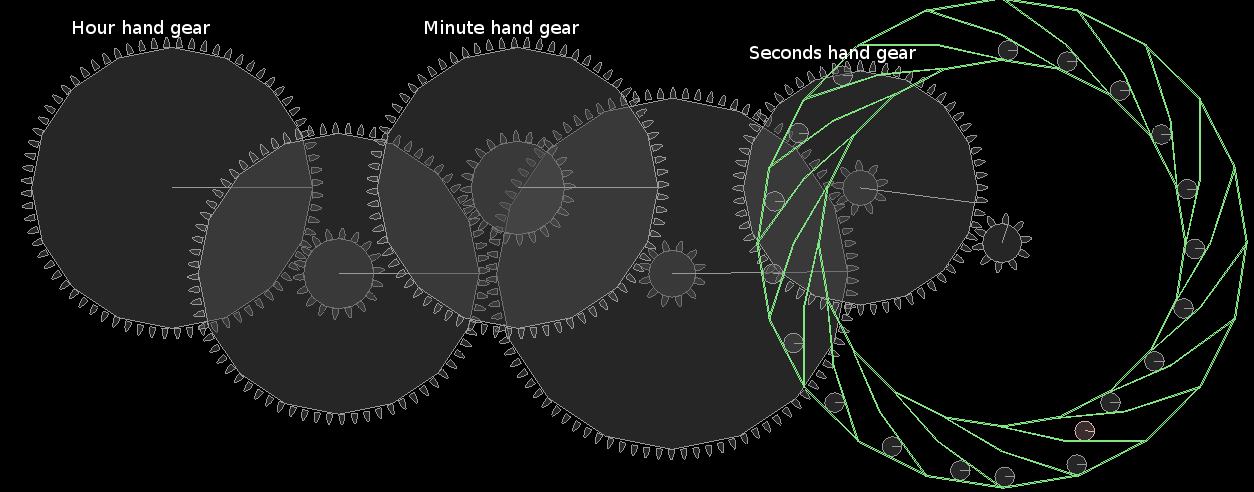
\includegraphics[width=0.7\textwidth]{images/clock.png}
\caption{Our Gear Clock}
\end{figure}

\section{Original Design}
In our original design, we intended to have a perfect perpetual motion machine that drives the gear clock.

\begin{figure}[ht!]
\centering
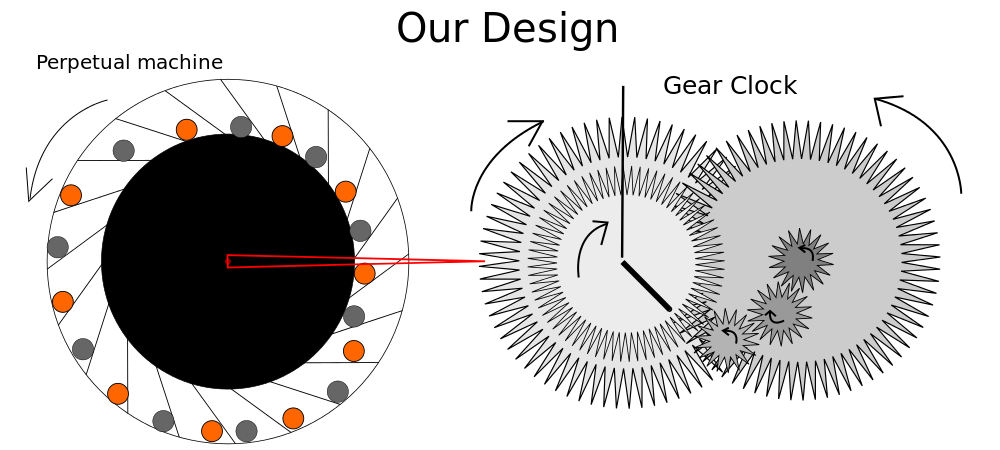
\includegraphics[width=0.7\textwidth]{images/project.png}
\caption{Our Original Design}
\end{figure}

\section{Final Design and Changes made in the original design}
In our final design, we added a motor to our perpetual wheel to move it at a constant angular velocity of \textit{pi/5 rad/sec}. We also moved the position of the gears to make them visible (Since they were of same size and would not be visible if one was over the other).

\begin{figure}[ht!]
\centering
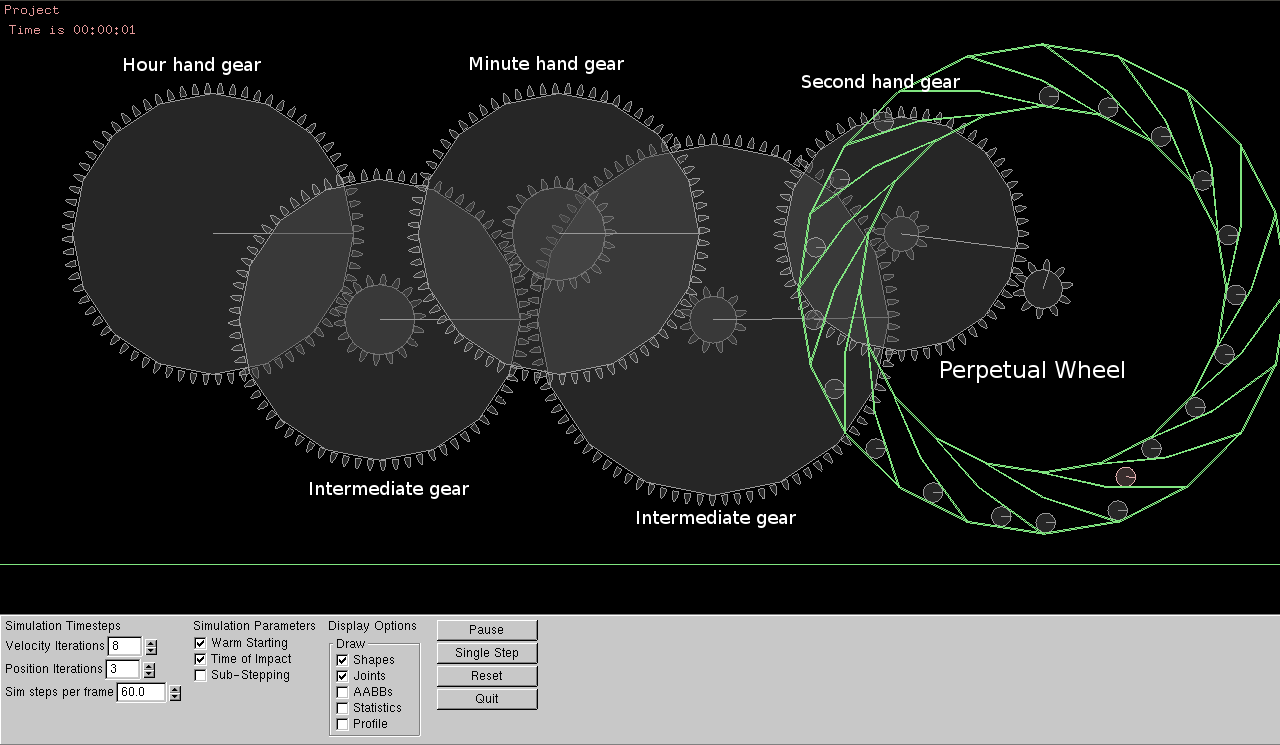
\includegraphics[width=0.7\textwidth]{images/final.png}
\caption{Our Final Design}
\end{figure}

\section{Reasons for modification of our original design}
We had tried lot of possible combinations of the dimensions (mass, radius, length, gravity) of each body of the perpetual wheel to make it move perpetually, but could not as we were bound to keep restitution of the bodies 0. This resulted in loss of energy and hence our wheel stopped rather earlier than expected. Hence, we added a motor to it to drive it at a uniform angular velocity.

\section{Analysis of code}
\subsection{Timing of the code}
Step time is the time taken for each iteration and the loop time is the total time taken for all the iterations since we are calculating the difference between the times of start of the loop and end of the loop to calculate the loop time. To calculate the step time we use an inbuilt function which gives the time taken for each step. Clearly the loop time is much larger than the step time because its is roughly the cumulative sum of the step times.\\
We analysed our code based on the average time taken over the number of iterations and plotted various graphs. We get a pretty uniform curve apart from the frequent spikes. This happens because after specific time intervals which denote the extra time taken for calculating the motion of the gears in the clock, due to contact/collisions. These are the graphs of the time taken for each step, velocity update, position update, collision update varied over the number of iterations.

\begin{figure}[ht!]
\centering
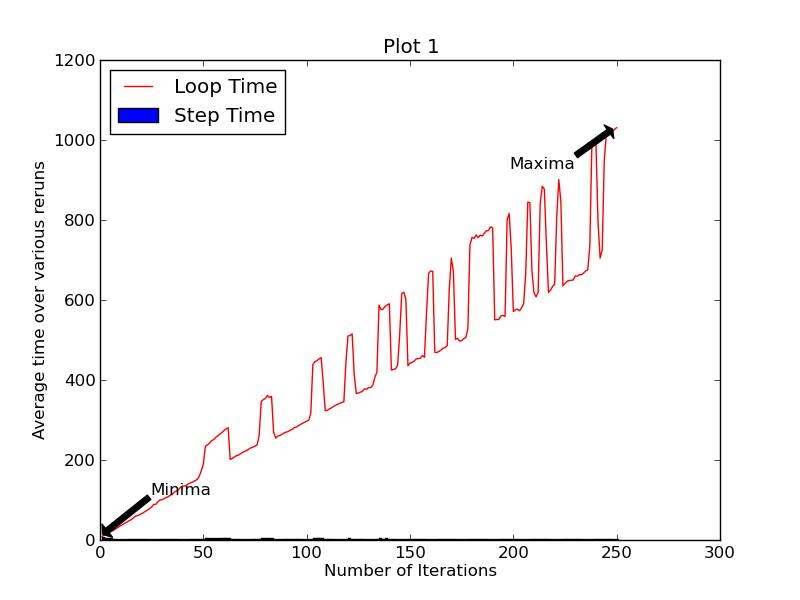
\includegraphics[width=0.5\textwidth]{images/plot1.jpg}
\caption{Plot of Average loop time vs No. of iterations}
\end{figure}
As seen in the first plot, the graph of step time is not even visible when plotted with the loop time. Also the loop time increases roughly with the increase in the number of iterations.

\begin{figure}[ht!]
\centering
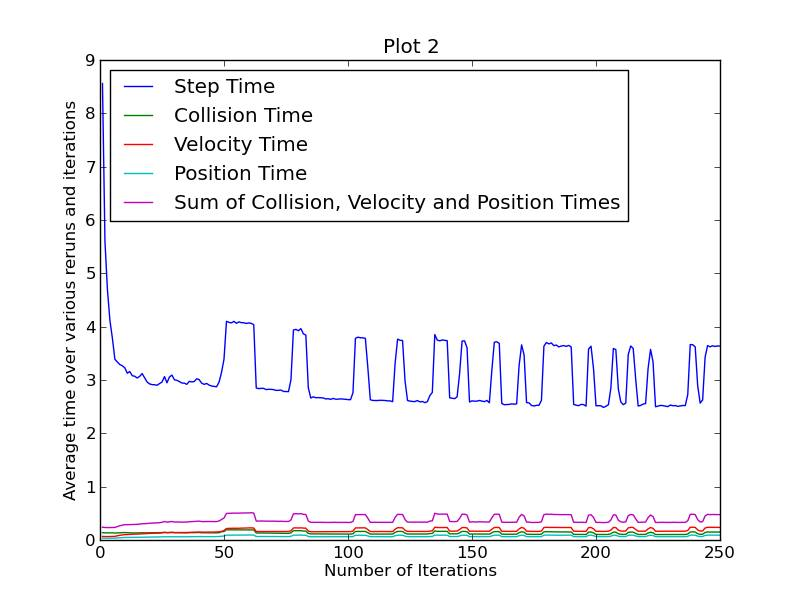
\includegraphics[width=0.5\textwidth]{images/plot2.jpg}
\caption{Plot of Average update time vs No. of iterations}
\end{figure}
Next, in plot 2 we plotted the Step time, collision time, velocity time, position time and the sum of collision, velocity and position time against the number of iterations. First interesting thing to notice is that the step time is very high till around the first 30 iterations. The reason behind it is the heavy functions called by Box2D to initialize the body, joint and fixture objects etc. and all the preprocessing that is done by Box2D for calculating the parameters (e.g AABB ,contact manifolds) which can be updated easily and are useful to make the simulation efficient in the future iterations.
\\
We also note that the velocity time is greater than the position time and collision time. This is because velocity iterations also involve the calculations and updates of some body parameters.

\begin{figure}[ht!]
\centering
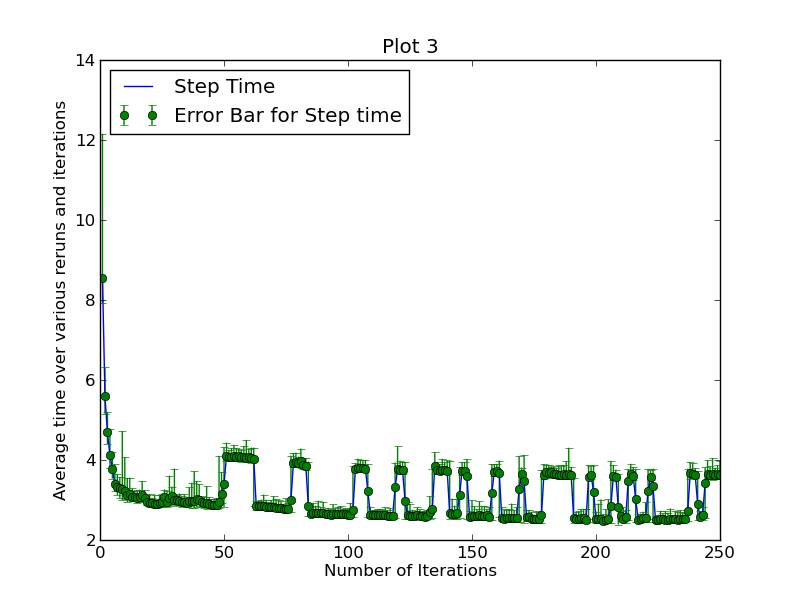
\includegraphics[width=0.5\textwidth]{images/plot3.jpg}
\caption{Plot of Frequency vs Time}
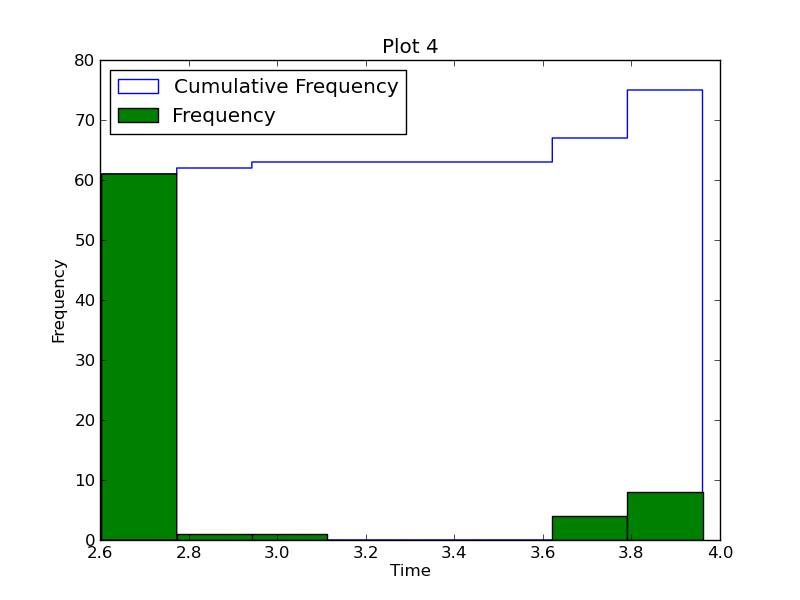
\includegraphics[width=0.5\textwidth]{images/plot4.jpg}
\caption{Plot of Average step time vs No. of iterations}
\end{figure}
Plot 3 and plot 4 were plotted for the error analysis of the data. In plot 3, we notice that the value of error is high initially,varies in between (even though the variations are very small they are noticeable) and becomes stable towards the end.This is due to the changing state of the CPU. Since we opened and closed different programs on the CPU while running the process, it shows the variations. In plot 4 we run the the simulation 84 times and analyse the step time for the 84\textsuperscript{th} iteration.

\begin{figure}[ht!]
\centering
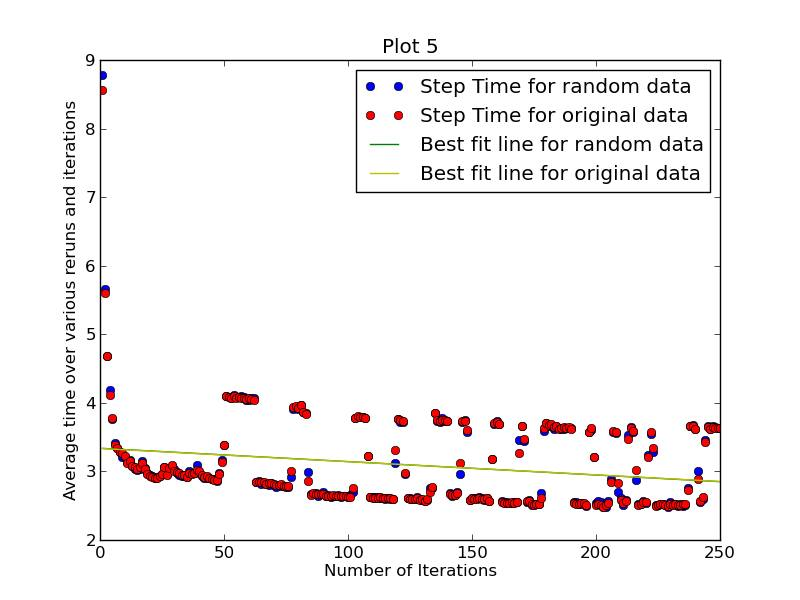
\includegraphics[width=0.5\textwidth]{images/plot5.jpg}
\caption{Plot of Average step time vs No. of iterations}
\end{figure}
Plot 5 was plotted taking random sample points to examine their values.

\subsection{Profiling}
We ran the simulation using different Box2D compile parameters, one using \textit{Release} and the other using \textit{Debug} mode and did Profile analysis for both methods.\\
We see that different functions take different proportion of the total time in the two modes. This is because in Release mode, the \textit{-O3} option along with \textit{g++} command optimises the run time, where 3 denotes the level of optimisation (i.e., -O3 does more optimisation than -O2), but sacrifices on the compile time. So if a function is called more number of times in the code, it will be a better candidate for optimisation, hence the difference in the proportion of time taken by each function in the two modes.\\
We also notice that the event count in \textit{Debug} mode is around 8 times the event count in \textit{Release} mode since the \textit{Debug} mode compiler additionally performs calls to debugging functions.

\begin{figure}[ht!] 
\centering 
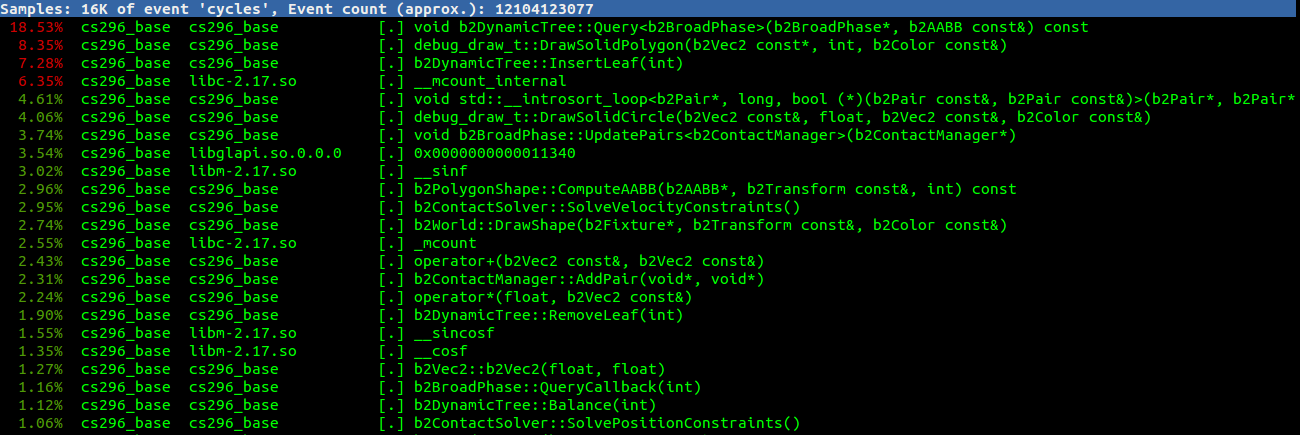
\includegraphics[width=1\textwidth]{images/release_mode.png} 
\caption{Proportion of total time taken by few processes in \textit{Release} mode (10,000 iterations)}
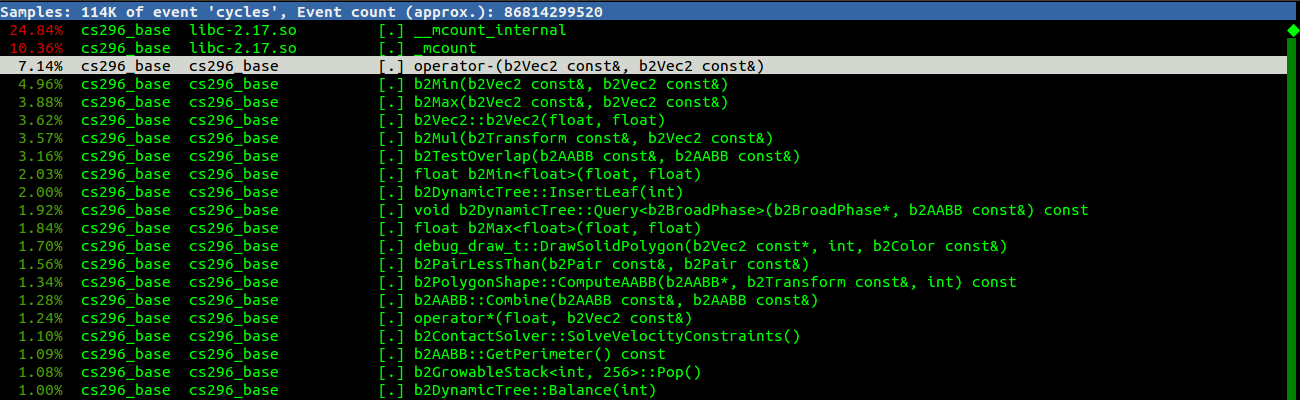
\includegraphics[width=1\textwidth]{images/debug_mode.png} 
\caption{Proportion of total time taken by few processes in \textit{Debug} mode (10,000 iterations)}
\end{figure}

From the above results, we infer that the function \textit{b2DynamicTree::Query\textless b2BroadPhase \textgreater(...)} takes the maximum proportion of the total loop time in Release mode, while the call to \textit{\_\_mcount\_internal} takes the maximum proportion of the total loop time in Debug mode.

\begin{figure}[ht!] 
\centering 
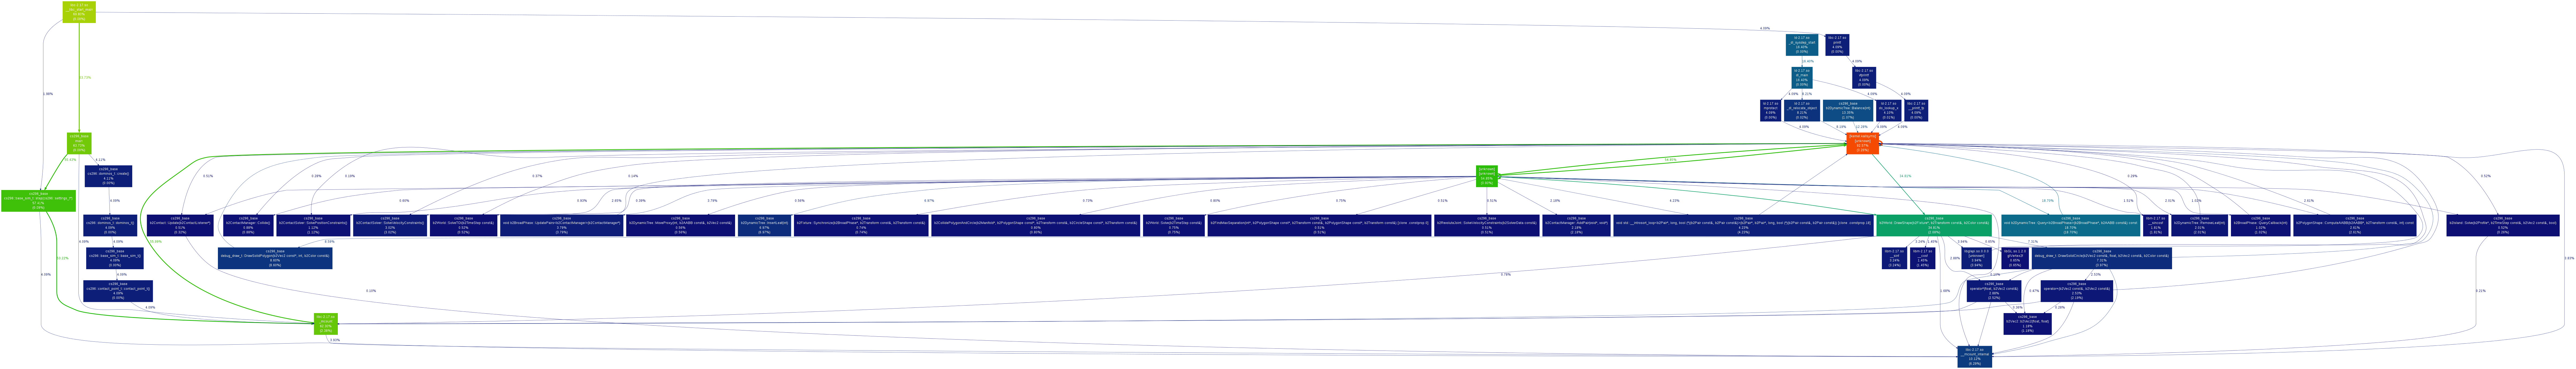
\includegraphics[width=1\textwidth]{images/release_cg.png} 
\caption{Call Graph for \textit{Release} mode : 10000 iterations}
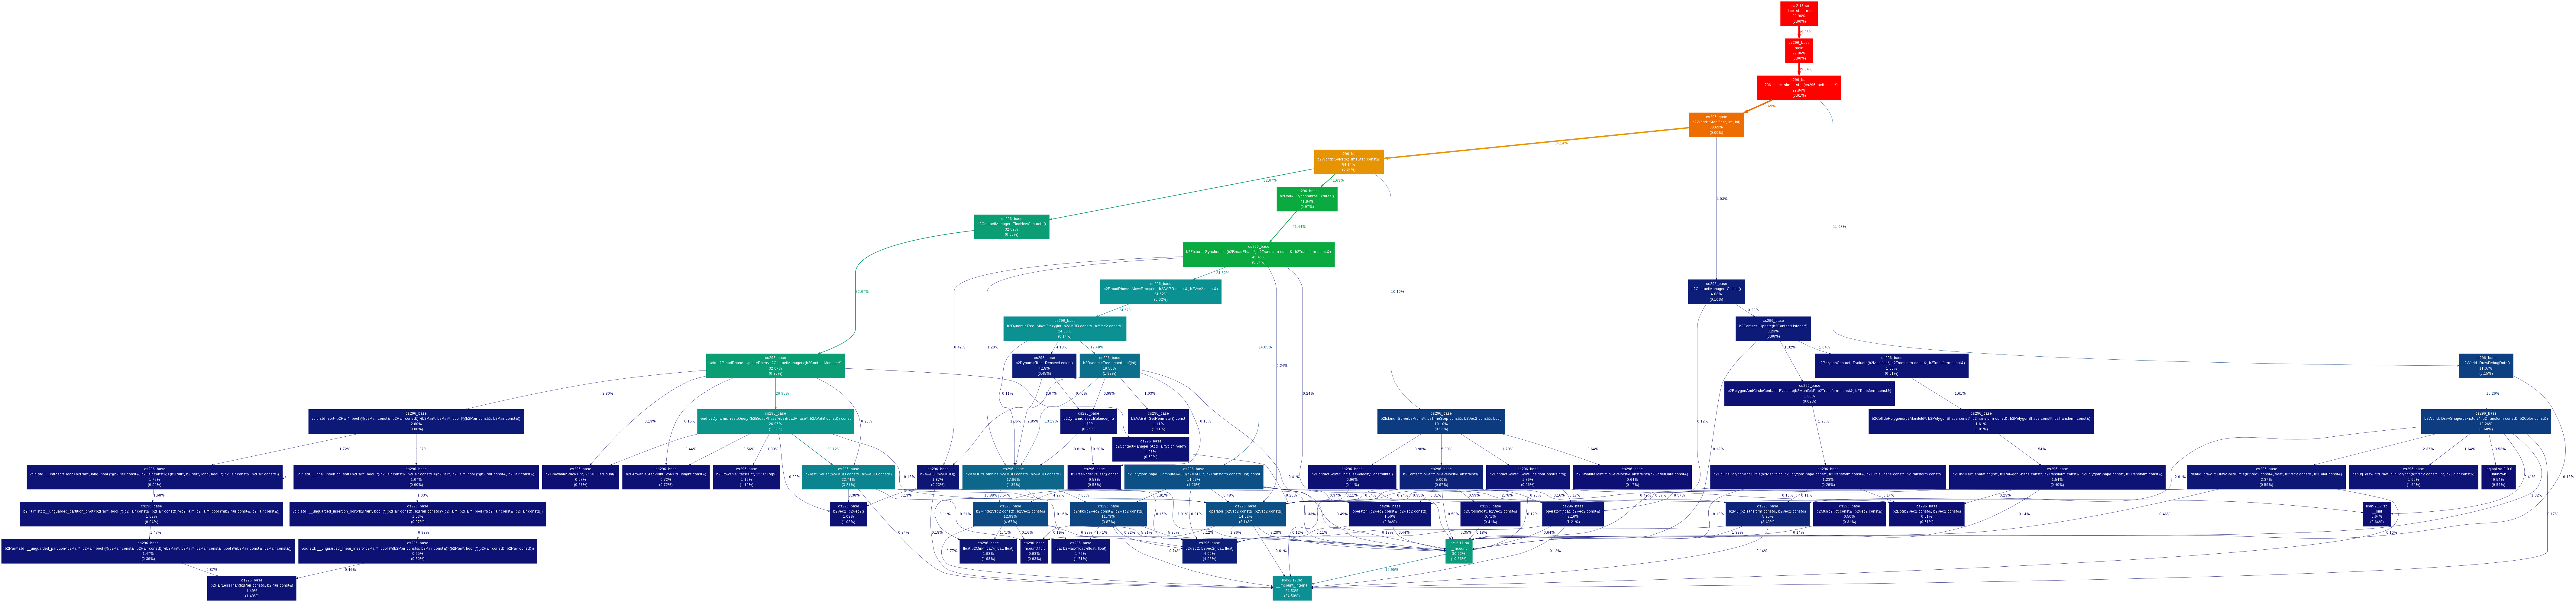
\includegraphics[width=1\textwidth]{images/debug_cg.png} 
\caption{Call Graph for \textit{Debug} mode : 10000 iterations}
\end{figure}
We observe that in general, the number of states/nodes in the call graph of the \textit{Debug} mode is greater than the number of states/nodes in the call graph of the \textit{Release} mode. This is because there was optimisation done in \textit{Release} mode, and also because extra calls to debugging functions are called because the mode is \textit{Debug}, which generates additional data to aid debugging.

\end{document}
